\documentclass[]{article}
\usepackage[margin=3cm]{geometry}
\usepackage{graphicx}
\usepackage{subcaption}
\usepackage{float}
\usepackage{amsmath}
\usepackage{enumerate}
\usepackage{amsmath}
\usepackage{bm}
\usepackage[linesnumbered,ruled,vlined]{algorithm2e}
% custom commands %
\newcommand{\half}{\frac{1}{2}}
\newcommand{\dd}{\textnormal{d}}
\newcommand{\ddx}{\frac{\dd}{\dd x}}
\newcommand{\dydx}{\frac{\dd y}{\dd x}}
\newcommand{\bfx}{\textbf{x}}
\newcommand{\bfR}{\textbf{R}}
%%% redefine eqnarray to not put equation numbering
\newenvironment{eq}
{\begin{eqnarray*}}
	{\end{eqnarray*}}
%%%

%opening
\title{A general simulated annealing approach to extracting nuclear dynamics from ultrafast x-ray scattering data}
\author{Thomas Northey}
\date{\today}

\begin{document}
	
	\maketitle
	
	\begin{abstract}
		abst
	\end{abstract}
	
	\section{Introduction}
	1m structure method \cite{yong2021determination}
	
	Some references \cite{yong2019scattering,yong2021determination,stankus2019ultrafast,wolf2019photochemical,moreno2019ab,northey2014ab,northey2016elastic}
	
	\subsection{Simulated annealing}
	
	Simulated annealing is a type of Metropolis algorithm, in that it always takes a downhill step while sometimes taking an uphill step \cite{press2007numerical}.
	
	It is a powerful tool in combinatorial minimisation, where the space over the which the function is defined is a discrete but very large configuration space. The size of the configurational space is factorially large, so that it cannot be explored exhaustively. Furthermore, since the set is discrete, we are deprived of any notion of continuing downhill in a favourable direction. The concept of direction may not have any meaning in the configuration space. A classic example of this is the travelling salesman problem.(taken from \cite{press2007numerical})
	
	
	The x-ray scattering signal is predominantly governed by the set of interatomic distances in any given molecule, as we know from the Debye model (independent atom model). The molecule itself moves along a continuous potential energy surface.
	
	
	\section{Method}
	
	\subsection{Simulated Annealing for molecules}
	
	\subsubsection{Theory}
	The molecular coordinates move iteratively according to,
	\[
	\textbf{R}_{i+1} = \textbf{R}_{i} + T_i\sum_{k=0}^{\textrm{modes}}a_k\hat{d}_k
	\]
	for temperature $T_i$ at iteration $i$, step-size $\Delta s$, displacement unit vectors $\hat{d}_k$, and wavenumbers $\omega_k$ for each normal mode. The factors $a_k$ are obtained from a uniform random distribution with range $\Delta s_k[-1, 1]$ to allow the molecule unconstrained movement along all its degrees of freedom.
	The motions are $\omega$-damped by the factor,
	\[
	w_k = \frac{\omega_0}{\omega_k}
	\]
	or
	\[
	w_k = \exp\Big(\frac{\omega_0}{\omega_k}\Big)
	\]
	for mode wavenumbers $\{\omega_0, \omega_1, \dots, \omega_n\}$, to avoid oversampling large motions of high frequency modes.
	
	The temperature decreases linearly at iteration $i$ as,
	\[
	%T_i = T_0\exp(-\gamma i / N)
	T_i = T_0(1 - i / N)
	\]
	for starting temperature $T_0\in(0, 1]$, and total iterations $N$.
	
	After each iteration, if the error function $\chi^2$ decreases the iteration is accepted
	\[
	i\rightarrow i+1
	\]
	If not, the iteration can still be accepted with probability,
	\[
	P = T_i
	\]
	which allows the molecule to sometimes travel uphill on the $\chi^2$ surface, thus escape local minima.
	\[
	\chi^2 = (x-y)^2
	\]
	If using multiple target and predicted data sources,
	\[
	\chi^2 = \sum_k A_k(x_k-y_k)^2
	\]


	\subsubsection{Algorithm}
	Current working strategy.
	
	\begin{itemize}
		
		\item	Low step-size (e.g.\ $\Delta s = 0.03$), large number of steps, multiple restarts (e.g.\ 10), last restart is a stochastic descent ($T_0 = 0$; greedy algorithm) starting from $\chi^2_\textrm{best}$.
		
		This usually finds very good starting time-steps, because the low step-size combined with large $N$ is very good at finding structures nearby to the starting geometry. That is, when the ring is starting to open.
		
		\item Subsequent runs with varying step-sizes (usually larger to find further away structures, $\Delta s = 0.05, 0.1, 0.2$) that load data from the previous run, and accept time-steps with $\chi^2 < \beta$, for e.g.\ $\beta = 10^{-5}$ or $10^{-6}$ (how low you can set the target depends on noise of data, in practice set it slightly lower than the best $\chi^2$ values of the first run). It will re-run time-steps starting from the previous `good' structures at earlier time. 
		
	\end{itemize}
	
	Assumption: the next best fit is `nearby' the previous step.
	
	\begin{itemize}
		\item Start at $\bfR(t_0)$, e.g.\ the optimised ground state geometry
		\begin{itemize}
			\item Start at $\bfR(t_j)$ and search for $\bfR(t_{j+1})$
			\item Perform $N$ temperature cycles ($T = T_0$), to allow a large search space around $\bfR(t_j)$
			\begin{itemize}
				\item Start at the end point of each cycle $\bfR_i$ to find the next cycle end point $\bfR_{i+1}$
				\item Save $\bfR_\textrm{best}$, the geometry with the lowest value of $\chi^2$
				
			\end{itemize}
		\end{itemize}
		
	\end{itemize}
	

	
	\section{Results}

	\subsection{CHD ring-opening example}
	
	\begin{figure}[H]
	\centering
	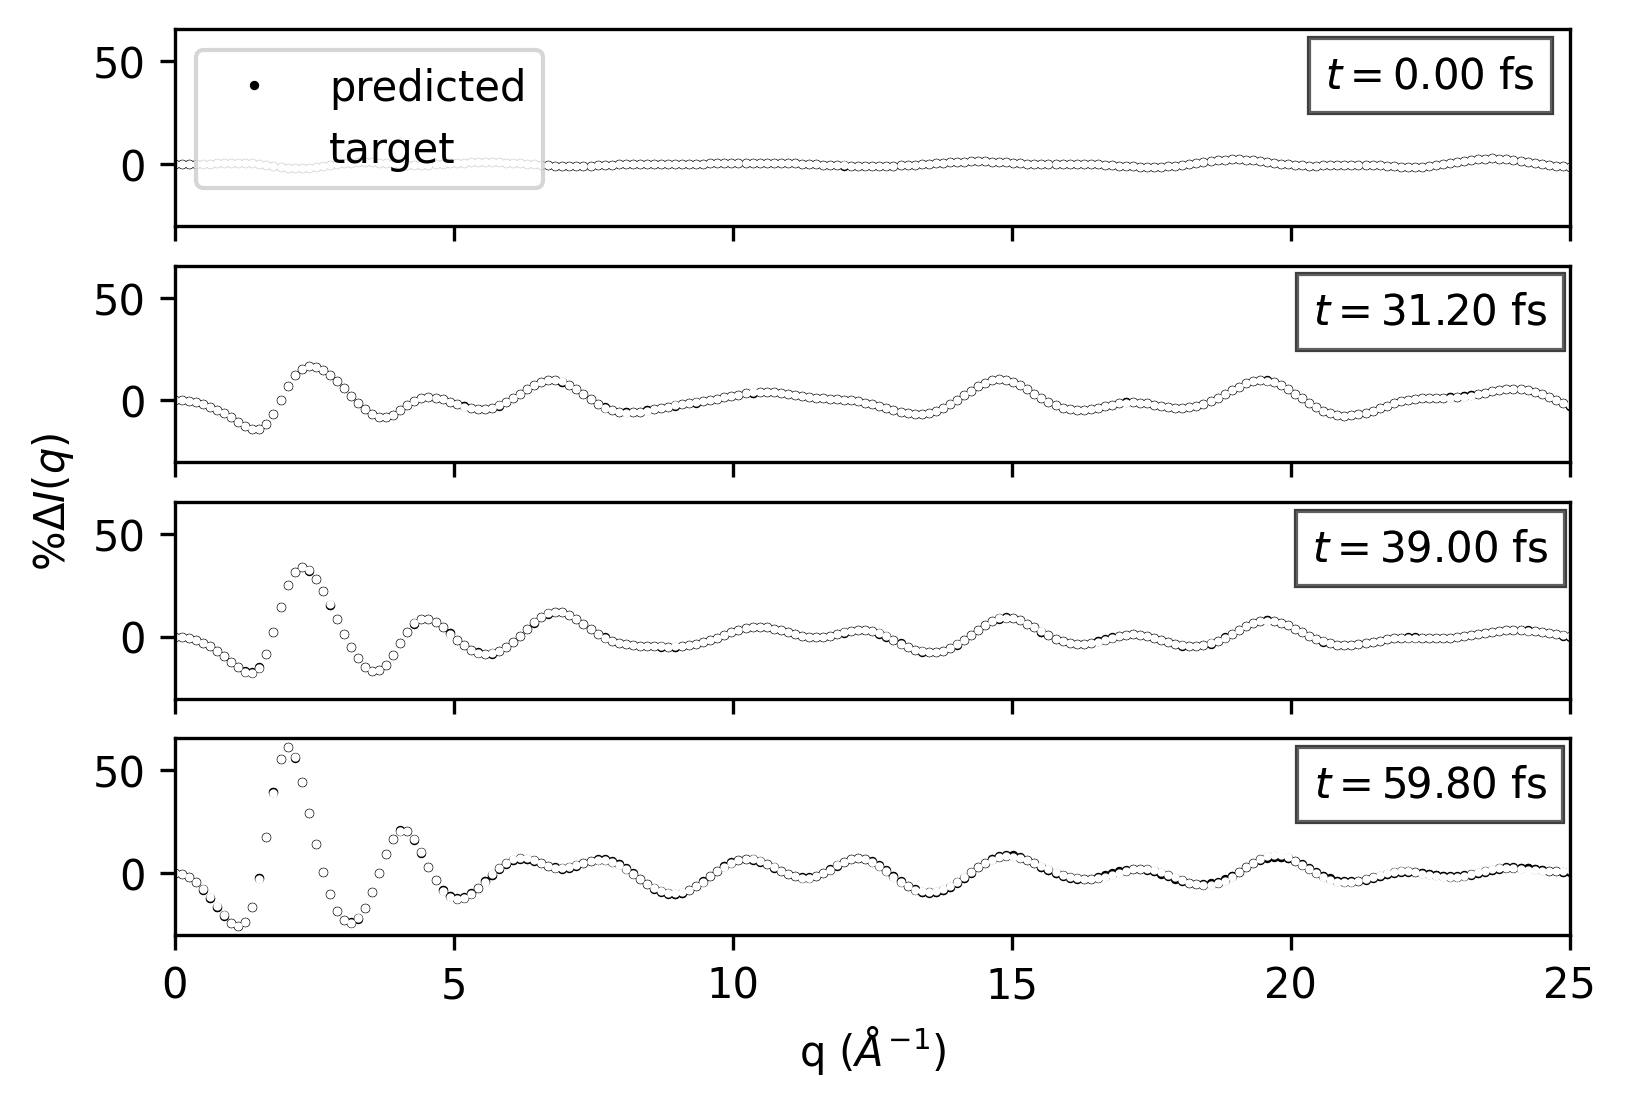
\includegraphics[width=0.8\textwidth]{lineouts.png}
	\caption{CHD x-ray scattering lineouts.}
	\end{figure}
	
	
	\begin{figure}[H]
		\centering
		\begin{subfigure}{0.8\textwidth}
		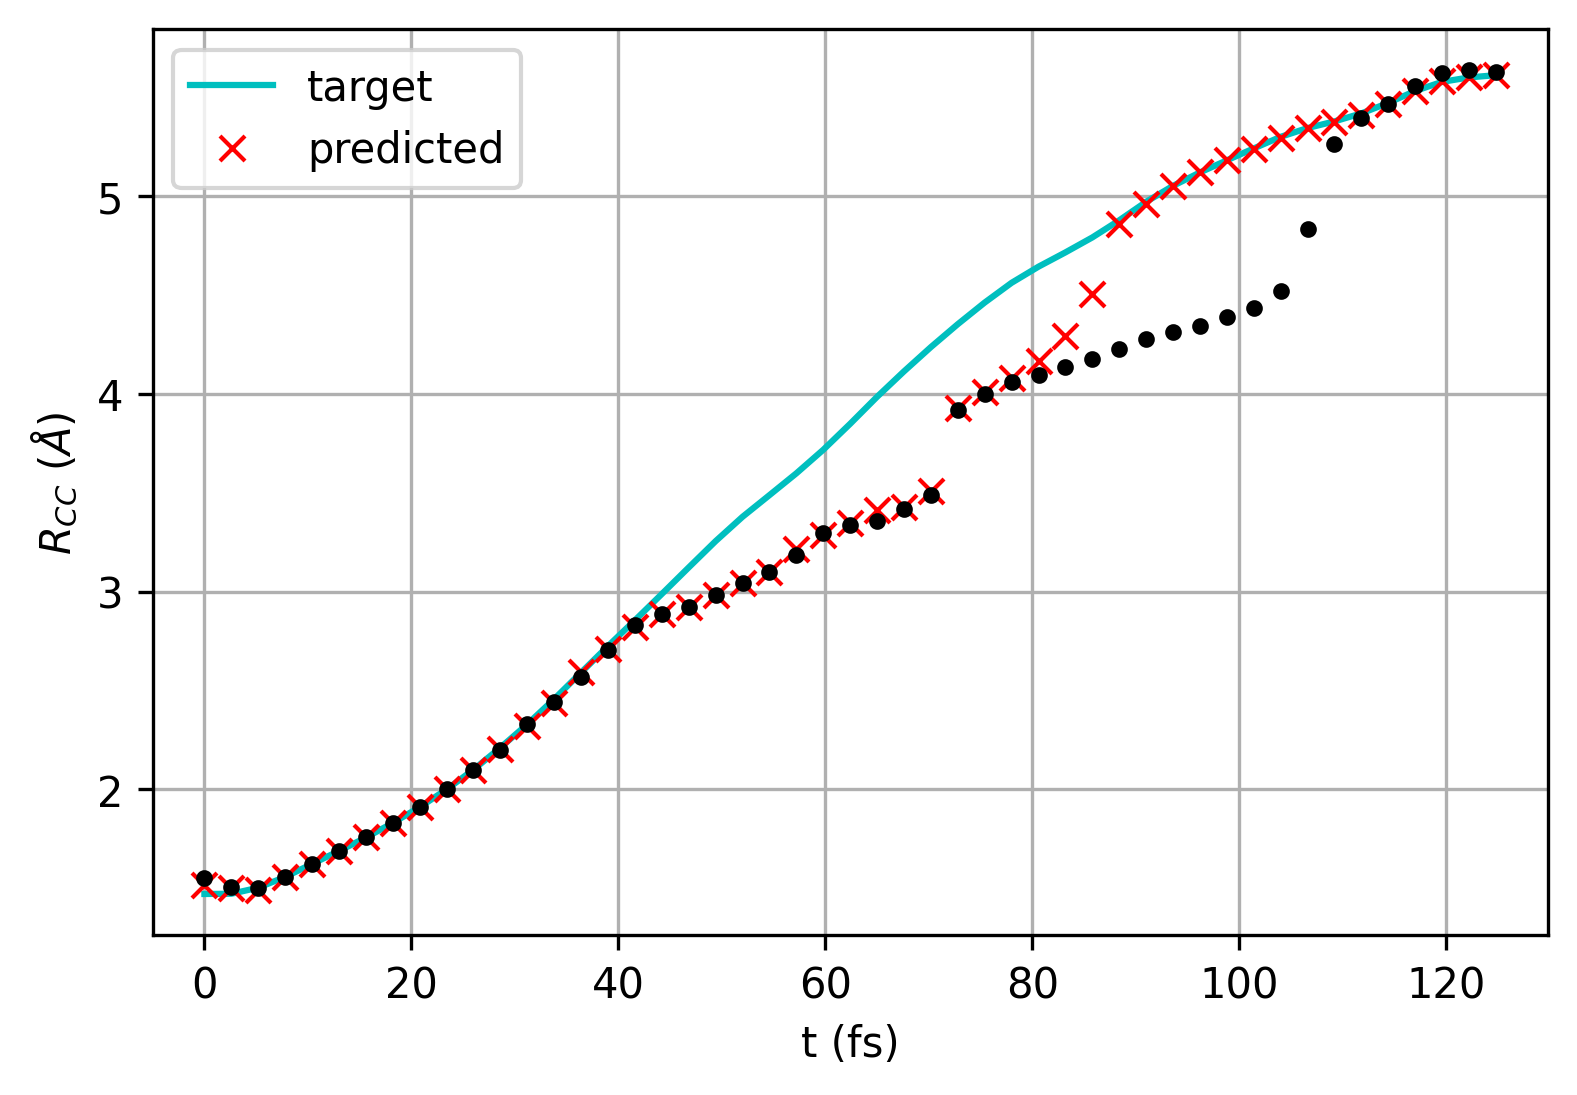
\includegraphics[width=\textwidth]{rcc_plots.png}
		\caption{Bond-opening C-C distance, and 1-3-4-6 dihedral angle.}
		\end{subfigure}
	\hfill
		\begin{subfigure}{\textwidth}
			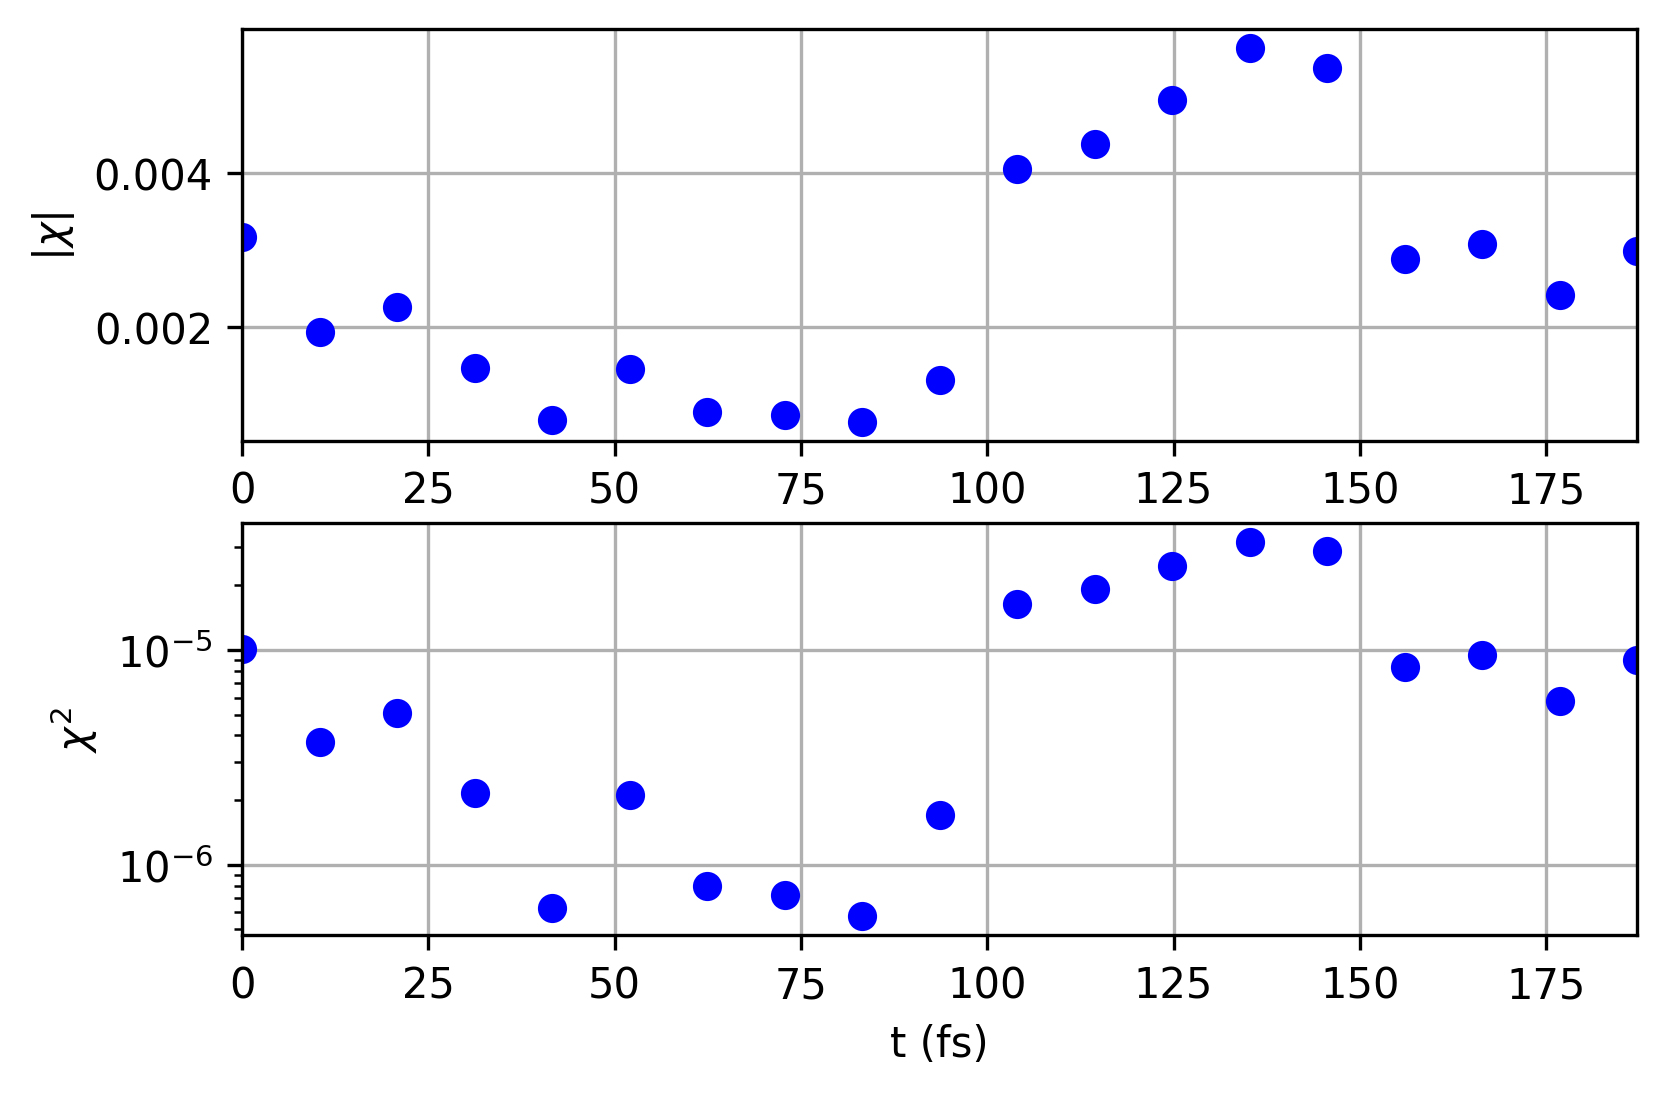
\includegraphics[width=0.8\textwidth]{chi2_t.png}
			\caption{$|\chi|$ and $\chi^2$ values for each time-point.u}
		\end{subfigure}
		\caption{CHD ring-opening C-C distance, $R_{CC}$. The target is from a surface hopping trajectory. Predictions are using $q_\textrm{max} = 12.0$ \AA$^{-1}$.}
		\label{fig:rcc_q25}
	\end{figure}

	\begin{figure}[H]
	\centering

		\begin{subfigure}{0.6\textwidth}
			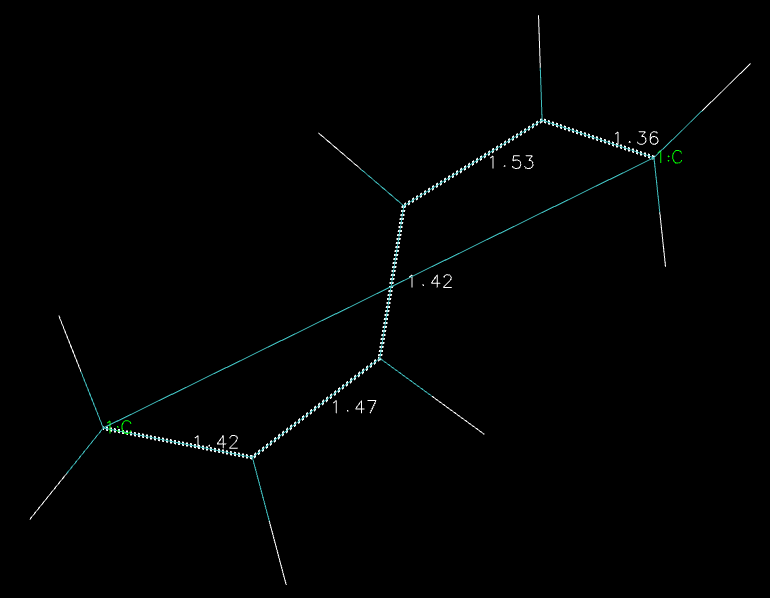
\includegraphics[width=\textwidth]{target_step48.png}
			\caption{Target.}
			\label{fig:chd_target}
		\end{subfigure}
	\hfill
		\begin{subfigure}{0.6\textwidth}
			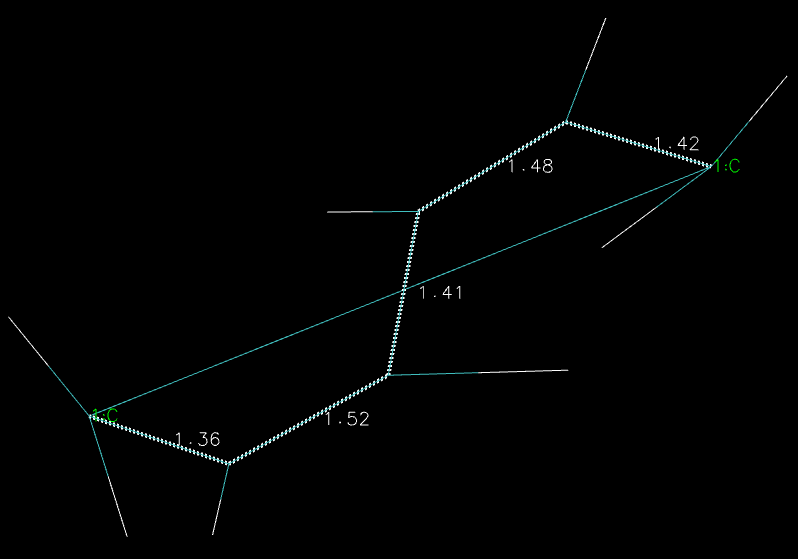
\includegraphics[width=\textwidth]{1003.png}
			\caption{Predicted.}
			\label{fig:chd_predicted}
		\end{subfigure}
	\caption{CHD target and predicted, showing all C-C bond-lengths.}
	\label{fig:figures}
	\end{figure}

	\subsection{Reproduce NMM trajectory from experiment data}
%\subsection{R 094}
%
%At first I try step-size 0.04, starting temperature 0.2. A lot of restarts e.g. 20-30 with about 900 steps (not accepted steps, just steps), 2 reverts followed by a restarting stochastic descent from $\chi^2_{\textrm{best}}$.

%\begin{figure}[H]
%	\centering
%	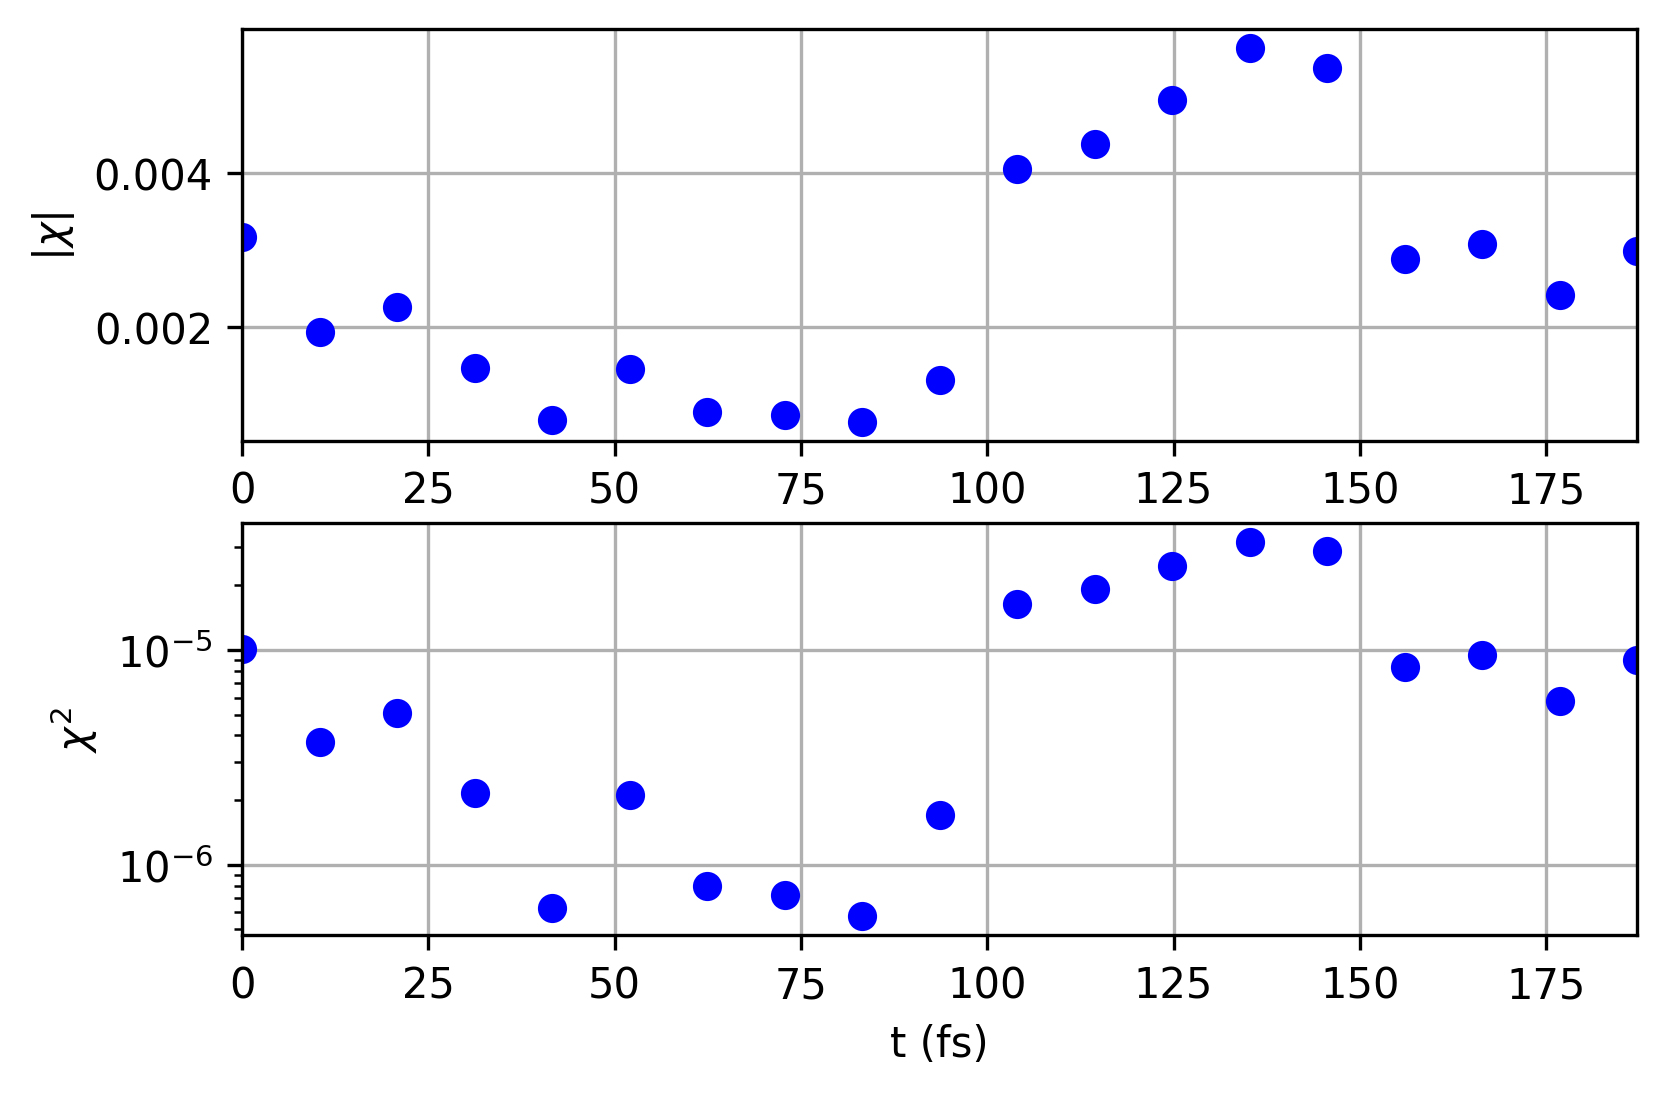
\includegraphics[width=0.8\textwidth]{chi2_t.png}
%	\caption{
	%Notes: It performs very well during step 0-14. I assume the minimum is out of reach for the algorithm at step 15. The sudden jump seems to reveal this...\\
	%Notes: Run starting at t=15 with more restarts (30 instead of 20). Same thing happens; it still can't find a low minimum...\\
	%Start at t=15 again. Increased step-size to 0.1, restarts back to 20. Ok it seems like it's a step-size issue. It strongly seems like the original runs cannot reach the lower minimum due to too small a step-size.\\
	%Again, more steps $N = 1429$. Performs similarly. The xyz file looks close to correct however; maybe $\chi^2 \sim 10^{-3}$ is acceptable.\\
	%Time-dependent step-size; proportional to the mean of the absolute target percent different signal. Performs badly.\\
	%Not shown: t-dependent $\Delta s$ but proportional to the delta between target pcd. Sometimes has very low, step-sizes = performs bad at later steps.\\
	%Not tried yet: step-size finder...\\
	%\\
	%Load previous npz file, and start from those xyzs. It will auto-skip ones with $\chi^2 < value$, and try to improve on others.
%	}

%\end{figure}


\bibliographystyle{plain}
\bibliography{library}
	
\end{document}
